\section{Datenbanken — Grundlagen}
\subsection{Datenbank – Definition}
Eine Datenbank speichert eine Vielzahl von Daten nach einem bestimmten Datenbankmodell. Im Gegensatz zu einem einfachen Verzeichnis werden die Daten strukturiert und redundanzfrei gespeichert. Außerdem ermöglicht eine Datenbank die dauerhafte (persistente) Speicherung von Daten.
\subsection{Datenbank-Management-System – DBMS}
Eine Datenbank wird immer durch ein Datenbank-Management-System (DBMS) verwaltet. Beispiele dafür sind MySQL, PostgreSQL oder Microsoft SQL Server. Das DBMS ist die Schnittstelle zur Datenbank – egal ob per CLI oder über eine GUI. Außerdem ermöglicht ein DBMS den Mehrnutzerbetrieb.

\begin{procon}
  \pro{Redundanzfreiheit -- Daten werden nur einmal gespeichert}
  \pro{Flexibilität -- Struktur lässt sich nachträglich anpassen}
  \pro{Physische Datenunabhängigkeit -- Anwendung ist von der Speicherform getrennt}
  \pro{Mehrnutzerbetrieb -- mehrere Nutzer können gleichzeitig zugreifen}
  \pro{Datenintegrität -- Konsistenz wird durch das DBMS sichergestellt}
  \pro{Recovery -- Wiederherstellung nach einem Fehler oder Absturz}
  \pro{Zugriffskontrolle -- Rechte können nutzerspezifisch vergeben werden}
  \con{Ressourcenintensiv -- benötigt mehr Rechenleistung und Speicher}
  \con{Komplexität -- Einrichtung und Administration erfordern Fachwissen}
  \con{Kosten -- Anschaffung, Lizenzen und Wartung verursachen laufende Ausgaben}
  \con{Schulungsaufwand -- Mitarbeiter müssen im Umgang mit dem DBMS geschult werden}
  \con{Single Point of Failure -- fällt das DBMS aus, sind alle Daten nicht verfügbar}
\end{procon}

\subsubsection{Anforderungen an ein DBMS}
\begin{enumerate}[leftmargin=*]
  \item \textbf{Redundanzabbau:} Durch Normalisierung verwaltet das DBMS die Daten so, dass sie möglichst wenig redundant gespeichert werden.
  \item \textbf{Datenintegrität:} Die gespeicherten Daten müssen korrekt und zuverlässig sein.
  \item \textbf{Effizienz und Performance:} Daten sollen schnell abgefragt werden können.
  \item \textbf{Benutzerfreundlichkeit:} Tabellen sollten verständlich benannt sein, damit Daten leicht zu finden sind und in sinnvollen Datentypen vorliegen.
  \item \textbf{Mehrfachzugriff:} Mehrere Nutzer sollen gleichzeitig auf die Datenbank zugreifen können.
  \item \textbf{Datenschutz:} Daten werden durch Nutzerrollen und Anonymisierung geschützt.
  \item \textbf{Datensicherheit:} Daten werden durch Backups gesichert und geschützt.
  \item \textbf{Datenunabhängigkeit:} Grad, in dem Nutzer und Anwendung unabhängig von der konkreten Speicherform auf das DBMS zugreifen können.
\end{enumerate}
\subsubsection{Aufbau eines DBMS}
\begin{figure}[H]
    \centering
    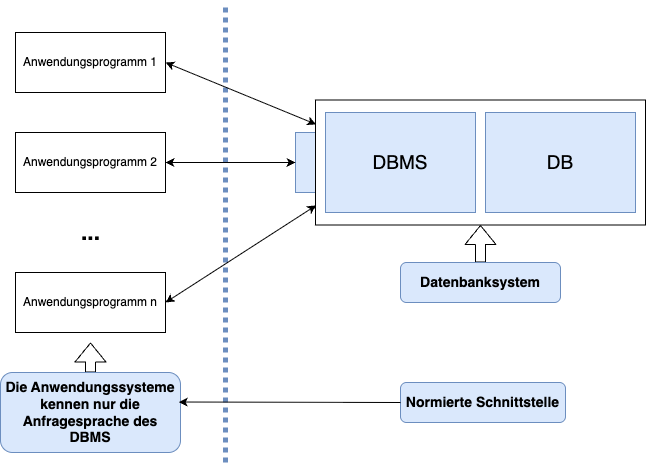
\includegraphics[width=\textwidth]{assets/images/DBMS-Aufbau}
    \caption{Aufbau eines DBMS}
\end{figure}
Auch bei dem Aufbau kann man Elemente wie den Mehrnutzerzugriff erkennen. Auch die Datenunabhängigkeit wird gezeigt, da die Anwendung nur die Anfragesprache kennt, aber nicht die Datenbank. Die Anfragesprache ist meist ein SQL-Dialekt.

\newpage